\documentclass{beamer}
\usepackage[utf8]{inputenc}

\usetheme{Madrid}
\usecolortheme{default}
\usepackage{amsmath,amssymb,amsfonts,amsthm}
\usepackage{txfonts}
\usepackage{tkz-euclide}
\usepackage{listings}
\usepackage{adjustbox}
\usepackage{array}
\usepackage{tabularx}
\usepackage{gvv}
\usepackage{lmodern}
\usepackage{circuitikz}
\usepackage{tikz}
\usepackage{graphicx}

\setbeamertemplate{page number in head/foot}[totalframenumber]

\usepackage{tcolorbox}
\tcbuselibrary{minted,breakable,xparse,skins}



\definecolor{bg}{gray}{0.95}
\DeclareTCBListing{mintedbox}{O{}m!O{}}{%
	breakable=true,
	listing engine=minted,
	listing only,
	minted language=#2,
	minted style=default,
	minted options={%
		linenos,
		gobble=0,
		breaklines=true,
		breakafter=,,
		fontsize=\small,
		numbersep=8pt,
		#1},
	boxsep=0pt,
	left skip=0pt,
	right skip=0pt,
	left=25pt,
	right=0pt,
	top=3pt,
	bottom=3pt,
	arc=5pt,
	leftrule=0pt,
	rightrule=0pt,
	bottomrule=2pt,
	toprule=2pt,
	colback=bg,
	colframe=orange!70,
	enhanced,
	overlay={%
		\begin{tcbclipinterior}
			\fill[orange!20!white] (frame.south west) rectangle ([xshift=20pt]frame.north west);
	\end{tcbclipinterior}},
	#3,
}
\lstset{
	language=C,
	basicstyle=\ttfamily\small,
	keywordstyle=\color{blue},
	stringstyle=\color{orange},
	commentstyle=\color{green!60!black},
	numbers=left,
	numberstyle=\tiny\color{gray},
	breaklines=true,
	showstringspaces=false,
}
%------------------------------------------------------------
%This block of code defines the information to appear in the
%Title page
\title %optional
{4.3.37}
%\subtitle{A short story}

\author % (optional)
{RAVULA SHASHANK REDDY - EE25BTECH11047}

 \begin{document}
	\frame{\titlepage}
	\begin{frame}{Question}
Find the equation of the line passing through the points  
\[
\vec{A} = \myvec{1 \\ 2}, 
\quad 
\vec{B} = \myvec{3 \\ 6}.
\]
\end{frame}
\begin{frame}{Equation}
Equation of a line is:
\begin{align*}
\vec{n}^T \vec{x} &= c 
    \end{align*}
\end{frame}
\begin{frame}{Theoretical Solution}
   \begin{align}
\myvec{\vec{A}&\vec{B}}^T\vec{n} &= \myvec{c\\c}\\
\myvec{\vec{A}&\vec{B}}^T\vec{n} &= \myvec{1\\1}\\
\myvec{1 & 2 \\ 3 & 6}\vec{n} &= \myvec{1 \\ 1}\\ 
\myvec{1 & 2 & 1 \\ 3 & 6 & 1} & 
\xrightarrow{R_2 - 3R_1}\;\;
\myvec{1 & 2 & 1 \\ 0 & 0 & -2} \\
0=-2
\end{align}
\begin{center}
Inconsistent.Hence c=0.
\end{center}

\begin{align}
\myvec{1 & 2  \\ 3 & 6 }\vec{n}= \myvec{0 \\ 0}\\
\end{align}

\end{frame}
\begin{frame}{Theoretical Solution}
\begin{align}
\myvec{1 & 2 & 0 \\ 3 & 6 & 0} & 
\xrightarrow{R_2 - 3R_1}\;\;
\myvec{1 & 2 & 0 \\ 0 & 0 & 0} \\
\vec{n} &= \myvec{-2 \\ 1}
\end{align}

Equation of a Line is
\begin{align}
\vec{n}^T \vec{x} &= c \\
\myvec{-2 & 1}\myvec{1 \\ 2} &= c \\
c &= 0 \\
\myvec{-2 & 1}\vec{x} &= 0 \\
-2x + y &= 0 \\
\boxed{y = 2x}
\end{align}
\end{frame}
\begin{frame}[fragile]
    \frametitle{C Code}
    \begin{lstlisting}
        #include <stdio.h>

int main() {
    // Points A and B
    int Ax = 1, Ay = 2;
    int Bx = 3, By = 6;

    // Direction vector of AB
    int dx = Bx - Ax;
    int dy = By - Ay;

    // Normal vector (perpendicular to direction)
    int nx = -dy;
    int ny = dx;

    // Equation: n^T * x = c
    // Compute c using point A
    int c = nx * Ax + ny * Ay;
\end{lstlisting}
\end{frame}
\begin{frame}[fragile]
    \frametitle{C Code}
    \begin{lstlisting}
    printf("Normal vector n = (%d, %d)\n", nx, ny);
    printf("Equation of line: %d*x + %d*y = %d\n", nx, ny, c);

    // Convert to slope-intercept form if ny != 0
    if (ny != 0) {
        double slope = -(double)nx / ny;
        double intercept = (double)c / ny;
        printf("Line equation (y = mx + c): y = %.2fx + %.2f\n", slope, intercept);
    }

    return 0;
}
    \end{lstlisting}
\end{frame}
\begin{frame}[fragile]
    \frametitle{Python Direct}
    \begin{lstlisting}
import numpy as np
import matplotlib.pyplot as plt
# local imports
from libs.line.funcs import *
from libs.triangle.funcs import *
from libs.conics.funcs import circ_gen

# Points
A = np.array([1, 2]).reshape(-1,1)
B = np.array([3, 6]).reshape(-1,1)

# Direction vector AB
d = B - A

# Normal vector n (perpendicular to AB)
n = np.array([-d[1,0], d[0,0]]).reshape(-1,1)
 \end{lstlisting}
\end{frame}
\begin{frame}[fragile]
    \frametitle{Python Direct}
    \begin{lstlisting}
# Compute c using point A
c = (n.T @ A)[0,0]

# Line equation: y = (c - n1*x)/n2
x_vals = np.linspace(0, 5, 100)
y_vals = (c - n[0,0]*x_vals)/n[1,0]

# Plot
plt.figure(figsize=(6,6))

# Line
plt.plot(x_vals, y_vals, 'b-', label='Line AB')

# Points with coordinates labeled
plt.plot(A[0,0], A[1,0], 'ro')  
plt.text(A[0,0]+0.1, A[1,0]+0.1, f'A({A[0,0]}, {A[1,0]})', fontsize=12, color='red')
 \end{lstlisting}
\end{frame}
\begin{frame}[fragile]
    \frametitle{Python Direct}
    \begin{lstlisting}
plt.plot(B[0,0], B[1,0], 'go')  
plt.text(B[0,0]+0.1, B[1,0]+0.1, f'B({B[0,0]}, {B[1,0]})', fontsize=12, color='green')

# Axes and grid
plt.xlabel('x')
plt.ylabel('y')
plt.title('Line through points A and B')
plt.grid(True)
plt.axis('equal')
plt.legend()
plt.show()
    \end{lstlisting}
\end{frame}
\begin{frame}[fragile]
    \frametitle{Python Shared Output}
    \begin{lstlisting}
    import ctypes
import numpy as np
import matplotlib.pyplot as plt
# local imports
from libs.line.funcs import *
from libs.triangle.funcs import *
from libs.conics.funcs import circ_gen

# Load C shared library
lib = ctypes.CDLL('./libline.so')

# Define argument and return types
lib.line_normal.argtypes = [ctypes.c_double, ctypes.c_double,
                            ctypes.c_double, ctypes.c_double,
                            ctypes.POINTER(ctypes.c_double),
                            ctypes.POINTER(ctypes.c_double),
                            ctypes.POINTER(ctypes.c_double)]
\end{lstlisting}
\end{frame}
\begin{frame}[fragile]
    \frametitle{Python Shared Output}
    \begin{lstlisting}
# Points
Ax, Ay = 1.0, 2.0
Bx, By = 3.0, 6.0

# Prepare output variables
n1 = ctypes.c_double()
n2 = ctypes.c_double()
c  = ctypes.c_double()

# Call the C function
lib.line_normal(Ax, Ay, Bx, By, ctypes.byref(n1), ctypes.byref(n2), ctypes.byref(c))
\end{lstlisting}
\end{frame}
\begin{frame}[fragile]
    \frametitle{Python Shared Output}
    \begin{lstlisting}
print("Normal vector n =", n1.value, n2.value)
print("Scalar c =", c.value)

# Line: y = (c - n1*x)/n2
x_vals = np.linspace(0, 5, 100)
y_vals = (c.value - n1.value * x_vals)/n2.value

# Plot
plt.figure(figsize=(6,6))
plt.plot(x_vals, y_vals, 'b-', label='Line AB')
\end{lstlisting}
\end{frame}
\begin{frame}[fragile]
    \frametitle{Python Shared Output}
    \begin{lstlisting}
# Points labeled with coordinates
plt.plot(Ax, Ay, 'ro')
plt.text(Ax+0.1, Ay+0.1, f'A({Ax}, {Ay})', fontsize=12, color='red')

plt.plot(Bx, By, 'go')
plt.text(Bx+0.1, By+0.1, f'B({Bx}, {By})', fontsize=12, color='green')

plt.xlabel('x')
plt.ylabel('y')
plt.title('Line through points A and B (computed via C + ctypes)')
plt.grid(True)
plt.axis('equal')
plt.legend()
plt.show()
 \end{lstlisting}
\end{frame}  
\begin{frame}{Plot}
    \begin{figure}
        \centering
        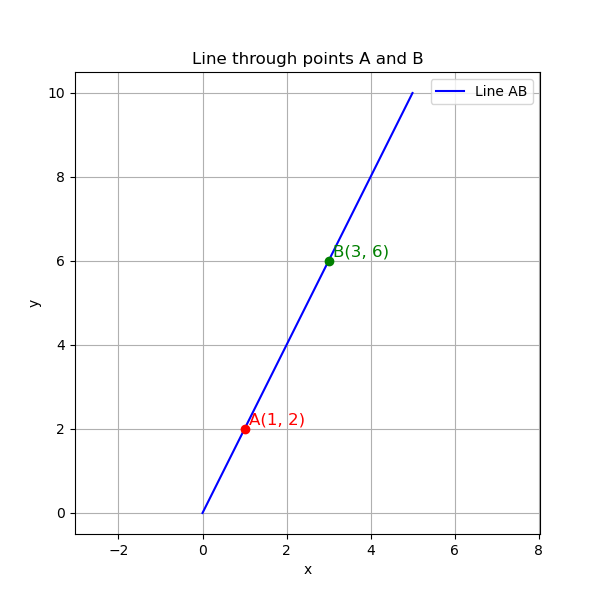
\includegraphics[width=1.0\linewidth]{figs/fig1.png}
        \caption{Caption}
        \label{fig:placeholder}
    \end{figure}
\end{frame}
\end{document}